% XeLatex-PDF
\documentclass[a4paper,11pt,phdthesis,singlespace,twoside]{cssethesis}

\usepackage{harvard} % Use the Harvard bibliography and citation package
\usepackage{graphicx}
\usepackage{epstopdf}
\usepackage{mathptmx}
\usepackage{times}

\usepackage{algorithm}
\usepackage{enumitem}

\usepackage{listings}
\usepackage{color}
\usepackage{apacite}

% Definitions needed by the cssethesis class. 
\thesisauthor{Viet Vo}
\thesisauthorpreviousdegrees{BSc., MSc.} % Optional
\thesisdepartment{Caulfield School of Information Technology}
\thesisauthorstudentid{26356988} % Needed for litreview
\thesisauthoremail{viet.vo\@@monash.edu} 

%\thesismonth{October} % Optional. Current month is used if this is not set
%\thesisyear{2015} % Optional. Current year is used if this is not set
\thesistitle{The Effects of Group Member's Parameters on Human Crowd Modelling}
\thesissupervisor{Prof. Bernd Meyer}
\thesissupervisoremail{bernd.meyer\@@monash.edu} 
\thesisassocsupervisor{Dr. Aldeida Aleti} 
\thesisassocsupervisoremail{aldeida.aleti\@@monash.edu} 
%\thesisdedication{I luv youse all} % Optional

% Set some preferences for the Harvard bibliography stuff 
% (See the documentation in harvard.ps)
%\citationstyle{dcu}
%\harvardparenthesis{round} % this can be round, square, curly, etc.
%\harvardyearparenthesis{round}

% start the document
\begin{document}

\frontmatter					% start the thesis front matter.

\thesistitlepage				% Generate the title page.
%\thesiscopyrightpage			% Generate the copyright page.
% \thesisdedicationpage			% Generate a dedication page (optional)
\tableofcontents				% Generate a table of contents.
\listoftables					% Generate a list of tables (optional).
\listoffigures					% Generate a list of figures (optional).

\begin{thesisabstract}			% generate the abstract page.
This thesis introduces \ldots
\end{thesisabstract}                 

%\thesisdeclarationpage			% generate the declaration page (optional).

%\begin{thesisacknowledgments}	% generate the acknowledgements page (optional).
%I would like to thank everyone who helped to make this possible. It has
%been an incredible journey of self-discovery, and I love every last one of
%you\ldots
%\end{thesisacknowledgments}   

%%%%%%%%%%%%%%%%%%%%%%%%%%%%%%%%%%%%%%%%%%%%%%%%%%%%%%%%%%%%%%%%%%%%%%%%%%%%%%
%%
%% Main matter 
%%
\mainmatter						% start the thesis body.

\chapter{Introduction}

Since over 70\% of the world population is predicted to live in cities by 2050 \cite{Weidmann2012}, rapid urbanization and population growth will be inevitable challenges in the effort of planning infrastructure, estimating traffic needs and capacities, and increasing the safety of pedestrians. With the increase in the number of public events and the number of accidents during these events since the crush disaster happened at the Station Nightclub, USA (2003) \cite{Evers2011}, the demand for realistic crowd simulation models becomes important for risk management in urban design and crowd safety. To develop realistic simulation models, various studies have been conducted in order to understand and simulate behaviours which can emerge in both normal and emergency situations such as groups of pedestrians moving with or competing against each other.

Group cohesion behaviour is the behaviour of objects moving towards the average positions of their neighbors over the time \cite{Reynolds1987}. The definition of this behaviour was motivated by the visual observation of coherently flying objects. The behaviour has been investigated widely on the collective motion of different flocking organisms including homing pigeon flocks \cite{Kattas2012}, fish schools \cite{Miller2013}, and bacteria colony \cite{Cisneros2007}. 

Human group cohesion behaviour is observed by its cohesion degree and formation. Cohesion degree denotes the average distance to the group’s centre of mass from each group member while observable human group formations are V-like, line-abreast, U-like, or river-like \cite {Helbing2005}. Group cohesion behaviour is important in both normal and evacuation scenarios. In normal situations, group cohesion behaviour can affect the speed and movement direction of pedestrians who are not belonging to any group. In human behaviour research, the frequency of group cohesion behaviour’s occurrence has been observed at different places in the UK with the percentages of 37\% at train station, 50\% at shopping centre, 28\% at university campus, 50\%, at Clumber Street \cite{Singh2009}. Pedestrians in the same group might be family members, colleagues. In crowd disasters, pedestrians evacuate with group rather than escape individually. Groups of families and friends with strong ties, stay together and evacuate together have been emphasized through socio-psychological research area \cite {Mawson2005}. They may move irrationally to maintain its cohesion and consequently become obstacles for other pedestrians \cite{Aguirre2011}.

%\chapter{Literature Review}
% often it is handy to keep the text of separate chapters in separate
% files, and then to read them into the master document, as here
\chapter{Literature Review}

In this chapter I will demonstrate some of the extended citation
capabilities provided by the {\sf Harvard} package \cite{WiS1994}. As well
as supporting the standard \LaTeX\ \verb+\cite+ command, it provides a
few other very useful ones.

The \verb+\cite+ command is best used when placing a citation at the end of
sentence or phrase (as above). When you want to refer to the authors of a
particular work, typically at the start of a sentence, \verb+\cite+ is not
appropriate. This is particularly so if you are using a numerical or
symbolic citation style. You should \emph{not} start a sentence with
\begin{quote}
[2] says that this is most certainly \ldots
\end{quote}
In such situations you really need to give the authors' names. The {\sf
Harvard} package provides a new command \verb+\citeasnoun+, which allows
you to produce things like:
\begin{quote}
\citeasnoun{Ade1983} describes a means by which textures may be
characterized \ldots another approach is given in \citeasnoun{DeV1998}.

\citeasnoun{AGR1996} note that humans have little or no difficulty in
perceiving shape, yet find it extremely difficult to \emph{describe} what
they perceive.
\end{quote}

Another useful new command provided by the {\sf Harvard} package is
\verb+\possessivecite+. This is used when you want to use the authors in a
possessive sense, as below:
\begin{quote}
\possessivecite{AGR1996} experiments with hundreds of three-dimensional scans of human heads suggests that \ldots
\end{quote}
Note that an abbreviated version of the authors' names has been used above.
The {\sf Harvard} package does this automatically after the first citation.
This behaviour can be overridden if desired.

\paragraph{Note:} The standard {\sf Harvard} package is incompatible with
\texttt{pdflatex} (via the {\sf html} package). If you want to use the {\sf
Harvard} package with \texttt{pdflatex}, make sure you use the version
supplied here (2.0.5a), which has been hacked to remove the problem.

In the long run, {\sf natbib} is probably the better choice. Watch this
space...
 % this causes a page-break, so put the \chapter
						% command in the file to be included - I don't know
						% why this happens :(

\chapter{Figures and Tables}
Here we will test that references to figures and tables work correctly.

\section{Figures}
\begin{figure}[ht]
\begin{center}
\resizebox{100mm}{!}{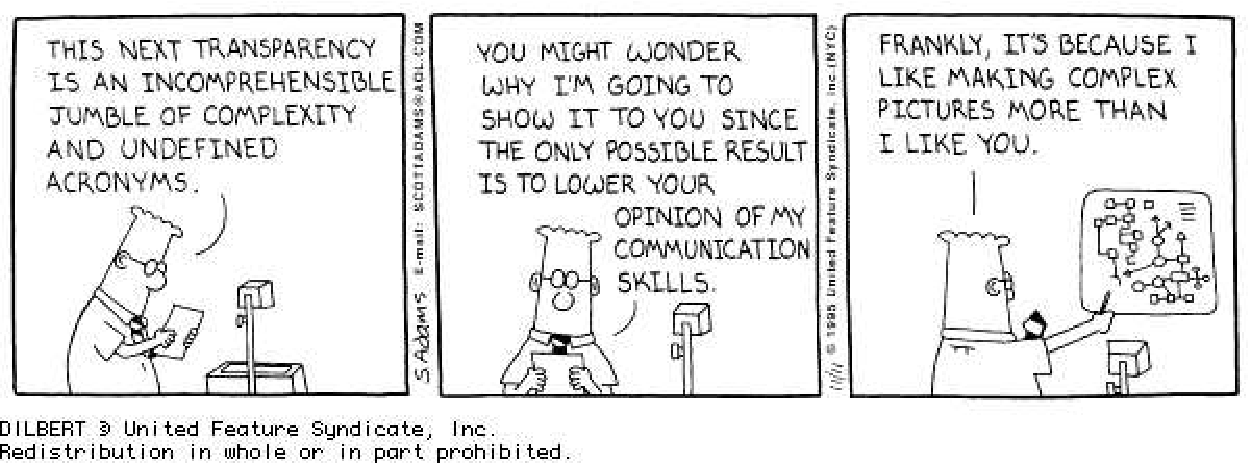
\includegraphics{dilbert_complexpictures}}
\end{center}
\caption{An example of a figure.}
\label{fig:example}
\end{figure}
See Figure~\ref{fig:example}.

\section{Tables}
\begin{table}
\begin{center}
\begin{tabular}{lcr}
23121 & 1212 & 232 \\ \hline  
cat & frog & dog
\end{tabular}
\end{center}
\caption{An example of a table}
\label{tab:example}
\end{table}
See Table~\ref{tab:example}.

\subsection{Referencing test}
See Table~\ref{tab:example} and Figure~\ref{fig:example}.

% another chapter
\chapter{Method AAAA}

\begin{figure}[H]
\begin{center}
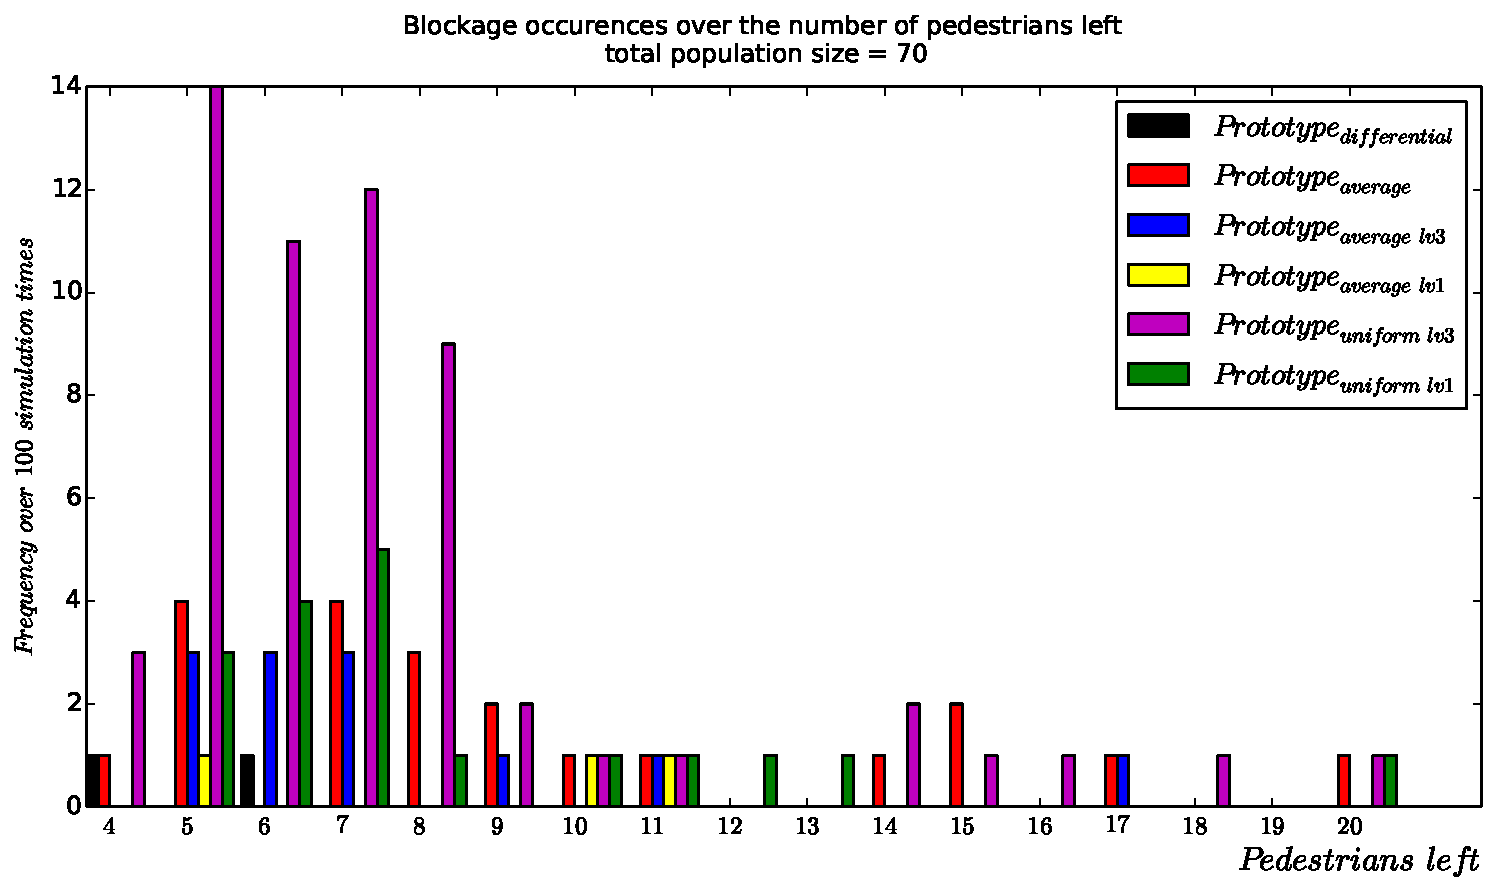
\includegraphics[width=0.2\columnwidth]{figs/blockage_frequency.pdf}
\end{center}
\caption{An example of a layered layout of a biological pathway with flow. The flow direction is left to right and this diagram has six vertical layers. Taken from http://www.pathwaycommons.org}
\label{fig:layeredflow}
\end{figure}

Lorem ipsum dolor sit amet, consetetur sadipscing elitr,  sed diam nonumy
eirmod tempor invidunt ut labore et dolore magna aliquyam erat, sed diam
voluptua. At vero eos et accusam et justo duo dolores et ea rebum. Stet clita
kasd gubergren, no sea takimata sanctus est Lorem ipsum dolor sit amet. Lorem
ipsum dolor sit amet, consetetur sadipscing elitr,  sed diam nonumy eirmod
tempor invidunt ut labore et dolore magna aliquyam erat, sed diam voluptua. At
vero eos et accusam et justo duo dolores et ea rebum. Stet clita kasd
gubergren, no sea takimata sanctus est Lorem ipsum dolor sit amet. Lorem ipsum
dolor sit amet, consetetur sadipscing elitr,  sed diam nonumy eirmod tempor
invidunt ut labore et dolore magna aliquyam erat, sed diam voluptua. At vero
eos et accusam et justo duo dolores et ea rebum. Stet clita kasd gubergren, no
sea takimata sanctus est Lorem ipsum dolor sit amet.

\begin{figure}[ht]
\begin{center}
\resizebox{100mm}{!}{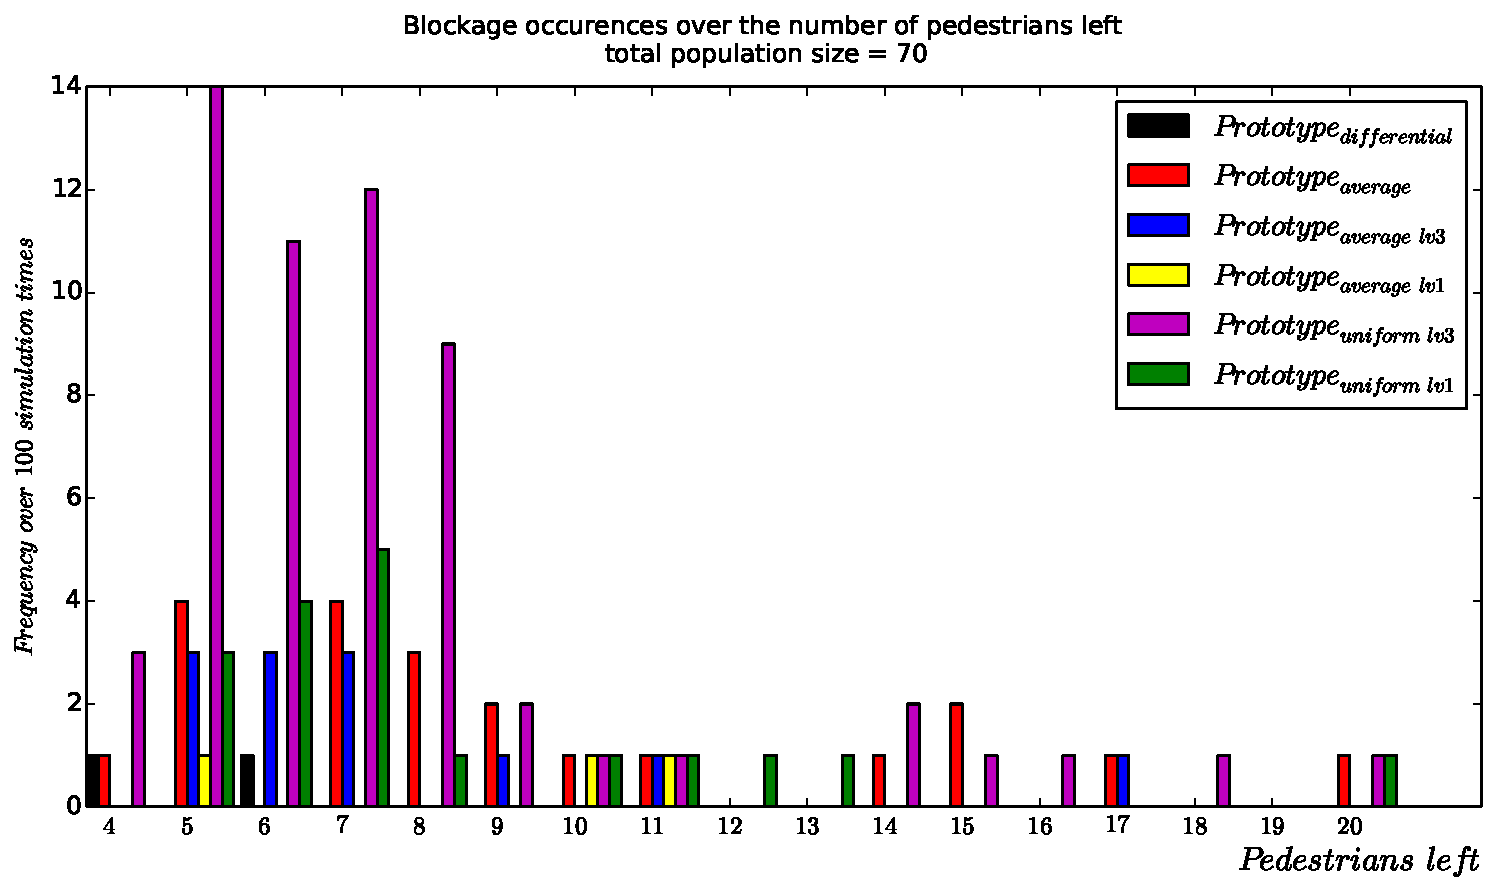
\includegraphics[width=0.05\columnwidth]{figs/blockage_frequency.pdf}}
\end{center}
\caption{An example of a figure.}
\label{fig:example}
\end{figure}

Duis autem vel eum iriure dolor in hendrerit in vulputate velit esse molestie
consequat, vel illum dolore eu feugiat nulla facilisis at vero eros et accumsan
et iusto odio dignissim qui blandit praesent luptatum zzril delenit augue duis
dolore te feugait nulla facilisi. Lorem ipsum dolor sit amet, consectetuer
adipiscing elit, sed diam nonummy nibh euismod tincidunt ut laoreet dolore
magna aliquam erat volutpat.


\appendix % all \chapter{..} commands after this will generate appendices

\chapter{This appendix should get a letter}
\label{app:example}
An appendix before the backmatter gets an automatically generated letter by
which it can be referred to. This is Appendix~\ref{app:example}.

\chapter{Simulation Source Code}
You may want to investigate the \texttt{lgrind} program and package if you
wish to include source code in your thesis

%%%%%%%%%%%%%%%%%%%%%%%%%%%%%%%%%%%%%%%%%%%%%%%%%%%%%%%%%%%%%%%%%%%%%%%%%%%%%%
%%
%% Back matter 
%%

%\backmatter						% start the thesis back matter
%\begin{thesisauthorvita}
%\begin{spacing}{1}
%Publications arising from this thesis include:
%\begin{description}
%\item[Author, A.\ and Bloggs, J.\ (2002),]
%A really catchy title. In \emph{The 31st International Conference
%on Non-specific Computing.} Capital City, Country.
%\item[Bloggs, J.\ and Author , A. (2002),]
%A very much longer and significantly less catchy title. in \emph {Workshop on
%A Research Area}. Springfield, USA.
%\end{description}
%\end{spacing}
%\end{thesisauthorvita}

\backmatter						% start the thesis back matter
%\begin{thesisauthorvita}
%\begin{spacing}{1}
%Publications arising from this thesis include:
%\begin{description}
%\item[Author, A.\ and Bloggs, J.\ (2002),]
%A really catchy title. In \emph{The 31st International Conference
%on Non-specific Computing.} Capital City, Country.
%\item[Bloggs, J.\ and Author , A. (2002),]
%A very much longer and significantly less catchy title. in \emph {Workshop on
%A Research Area}. Springfield, USA.
%\end{description}
%\end{spacing}
%\end{thesisauthorvita}


\chapter{Last Thing} % Appendices after the \backmatter
This sort of appendix has no letter. 

\bibliographystyle{apacite}
%\bibliographystyle{dcu} % A good style to use with the Harvard package
\bibliography{confirmationmonashbib}



\end{document}
